\documentclass[12pt, letterpaper]{article}

% ==========================================
%              DOCUMENT PACKAGES
% ==========================================

% --- Core Language & Encoding ---
\usepackage[english]{babel} % Sets the language and regional settings for English documents
\usepackage[utf8]{inputenc} % Allows the use of UTF-8 characters in the document
\usepackage[T1]{fontenc} % Specifies the font encoding
\usepackage[margin=2cm]{geometry} % Sets the page margins

% --- Colors & Graphics ---
\usepackage[table,dvipsnames]{xcolor} % Advanced color management
% \usepackage{color} % Basic package for text and background colors
\usepackage{graphicx} % Enhanced support for including external images and scaling them
\usepackage{adjustbox} % Adjusts the size, scaling, and alignment of boxes, images, and tables
% \usepackage{background} % Allows adding background images or watermarks to pages
\usepackage{float} % Improves the interface for floating objects and adds the [H] placement
\usepackage{pdflscape} % Makes landscape pages display correctly on screen in PDF viewers
\usepackage{pdfpages} % Allows the inclusion of external multi-page PDF documents

% --- Math, Science & Engineering ---
\usepackage{amsfonts} % Provides extended mathematical fonts
\usepackage{amsmath} % Provides advanced mathematical typesetting and environments
\usepackage{amssymb} % Provides extended mathematical symbols
% \usepackage{amsmath, amssymb} % (Redundant combination line omitted for stability)
\usepackage{amsthm} % Facilitates the creation of theorem-like environments
\usepackage{mathtools} % Enhances amsmath with additional math tools and bug fixes
\usepackage{thmtools} % Extensions and customization options for theorem environments
\usepackage{nicematrix} % Enhances matrices and tabulars using PGF/TikZ
\usepackage{xy} % Typesets complex graphs and diagrams
\usepackage{circuitikz} % Allows drawing of electrical networks and circuits

% --- Typography & Fonts ---
\usepackage{avant} % Sets the default sans-serif font to Avant Garde
\usepackage{cantarell} % Sets the default sans-serif font to Cantarell
\usepackage{charter} % Sets the default roman font to Charter
\usepackage{cmbright} % Sets the font family to Computer Modern Bright 
\usepackage{helvet} % Sets the default sans-serif font to Helvetica
\usepackage{inconsolata} % Sets the default typewriter (monospace) font to Inconsolata
\usepackage{iwona} % Sets the font family to Iwona 
\usepackage{kurier} % Sets the font family to Kurier 
\usepackage{lmodern} % Loads the Latin Modern fonts 
\usepackage{textcomp} % Provides additional text symbols
\usepackage{ulem} % Provides various types of text underlining and strikethroughs

% --- Tables & Lists ---
\usepackage{array} % Extends the array and tabular environments
\usepackage{arydshln} % Allows dashed lines in arrays and tables
\usepackage{bigstrut} % Adds custom vertical space in table rows
\usepackage{booktabs} % Enhances the quality of tables with better horizontal rules
% \usepackage{colortbl} % Allows coloring of rows, columns, and individual cells in tables
\usepackage{diagbox} % Creates table cells with diagonal lines
\usepackage{enumitem} % Provides advanced control over list environments
\usepackage{longtable} % Allows tables to break across multiple pages
\usepackage{multirow} % Allows individual table cells to span across multiple rows
\usepackage{tabularx} % Creates tables with dynamically adjustable-width columns
\usepackage{pgfplotstable} % Reads and cleanly formats numerical tables directly from CSV

% --- Formatting, Layout & UI ---
\usepackage{blindtext} % Generates dummy text for testing document layouts
\usepackage{caption} % Customizes captions in floating environments
\usepackage{comment} % Allows you to block out large sections of text
\usepackage{emptypage} % Automatically removes headers and footers on empty pages
\usepackage{fancyhdr} % Allows complete customization of headers and footers
\usepackage{fancyvrb} % Enhanced verbatim environments for writing raw code
\usepackage{framed} % Creates framed, shaded, or differently highlighted text regions
\usepackage{fullpage} % Quickly sets all page margins to 1 inch
\usepackage{lipsum} % Generates Lorem Ipsum dummy text
\usepackage{mdframed} % Creates highly customizable framed environments
\usepackage{multicol} % Allows intermixing single and multiple text columns
\usepackage{parskip} % Replaces standard paragraph indentation with vertical spacing
\usepackage{setspace} % Controls line spacing (single, one-and-a-half, double)
\usepackage{subcaption} % Supports sub-figures and sub-tables with independent captions
% \usepackage{subfig} % Older package for sub-figures (subcaption is generally preferred now)
\usepackage{tcolorbox} % Creates heavily customized colored and framed text boxes
\usepackage{titlesec} % Customizes the formatting of section, subsection, and chapter headings
\usepackage{titling} % Provides advanced control over the typesetting of the document title

% --- Bibliographies & References ---
\usepackage{biblatex} % Advanced, modern bibliographic processing and formatting
\usepackage{csquotes} % Context-sensitive quotation facilities
\usepackage{makeidx} % Supports the generation of a document index
% \usepackage{natbib} % Flexible bibliography support, particularly for author-year citation styles

% --- TikZ & Plotting ---
\usepackage{tikz} % Advanced package for creating vector graphics and diagrams programmatically
\usepackage{pgf-pie} % Draws pie charts programmatically using PGF/TikZ
\usepackage{pgfplots} % Creates high-quality mathematical plots, charts, and graphs
% \usepackage{fancytikzposter} % Used to create large format academic posters using TikZ

% --- URLs & Hyperlinks ---
\usepackage{url} % Formats and properly hyphenates long URLs
\usepackage{breakurl} % Allows line breaks in URLs, especially when compiled with latex -> dvips
\usepackage{hyperref} % Creates cross-referencing, clickable links, and PDF bookmarks

% --- Code Formatting ---
\usepackage{listings} % Typesets programming source code with formatting and syntax highlighting


% ==========================================
%           DOCUMENT CONFIGURATION
% ==========================================

% Custom color definitions
\definecolor{mygray}{gray}{0.9}

% Hyperlink configuration
\hypersetup{
    colorlinks=true,
    linkcolor=blue,
    urlcolor=blue
}

% Configuración adicional para breaks en URLs
\def\UrlBreaks{\do\/\do-\do_\do.\do=\do?\do\&}
\expandafter\def\expandafter\UrlBreaks\expandafter{\UrlBreaks\do\a\do\b\do\c\do\d\do\e\do\f\do\g\do\h\do\i\do\j\do\k\do\l\do\m\do\n\do\o\do\p\do\q\do\r\do\s\do\t\do\u\do\v\do\w\do\x\do\y\do\z}

%Uncomment the following lines to use a sans-serif font
%\renewcommand{\familydefault}{\sfdefault}

% TikZ libraries
\usetikzlibrary{shapes.geometric, positioning, decorations.pathreplacing}

\graphicspath{ {./img/} } % Sets the path for the graphics

\newlist{biblio}{enumerate}{1}
\setlist[biblio,1]{label=[\arabic*]}

\makeindex

% \tiny
% \scriptsize
% \footnotesize
% \small
% \normalsize (default size)
% \large
% \Large
% \LARGE
% \huge
% \Huge

% ==========================================
%         GLOBAL LISTINGS SETTINGS
% ==========================================
\lstset{
basicstyle=\ttfamily\small,
numbers=left,
numberstyle=\tiny\color{gray},
stepnumber=1,
numbersep=10pt,
backgroundcolor=\color{white},
showspaces=false,
showstringspaces=false,
breaklines=true,
frame=single,
tabsize=2,
captionpos=b,
lineskip=-1pt,
extendedchars=true,
literate={á}{{\'a}}1 {é}{{\'e}}1 {í}{{\'i}}1 {ó}{{\'o}}1 {ú}{{\'u}}1 {Á}{{\'A}}1 {É}{{\'E}}1 {Í}{{\'I}}1 {Ó}{{\'O}}1 {Ú}{{\'U}}1 {ñ}{{\~n}}1 {Ñ}{{\~N}}1 {¿}{{\textquestiondown}}1 {¡}{{\textexclamdown}}1
}

% ==========================================
%            LANGUAGE: SQL
% ==========================================
\lstdefinestyle{sqlstyle}{
	language=SQL,
	keywordstyle=\color{blue}\bfseries,
	commentstyle=\color[rgb]{0,0.5,0}\itshape,
	stringstyle=\color{red}
}

% ==========================================
%            LANGUAGE: VHDL
% ==========================================
\lstdefinelanguage{VHDL}{
	morekeywords={entity, architecture, signal, port, in, out, inout, begin, end, process, if, then, else, elsif, case, when, others, for, while, loop, wait, library, use, std_logic, std_logic_vector, integer, boolean, rising_edge, falling_edge, component, generic, map, downto, to, and, or, not, xor, nand, nor, xnor},
	morecomment=[l]{--},
	morestring=[b]",
	sensitive=false,
	alsoletter={_}
}

\lstdefinestyle{vhdl}{
	language=VHDL,
	keywordstyle=\color{blue}\bfseries,
	commentstyle=\color[rgb]{0,0.6,0}\itshape,
	stringstyle=\color{red}
}

% ==========================================
%              LANGUAGE: C
% ==========================================
\lstdefinestyle{cstyle}{
	language=C,
	keywordstyle=\color{blue}\bfseries,
	commentstyle=\color[rgb]{0,0.5,0}\itshape,
	stringstyle=\color{red},
	directivestyle=\color{purple},
	tabsize=4 % Overrides the global tabsize of 2 for C code specifically
}

% ==========================================
%             LANGUAGE: C++
% ==========================================
\lstdefinestyle{cppstyle}{
	language=C++,
	keywordstyle=\color{blue}\bfseries,
	commentstyle=\color[rgb]{0,0.5,0}\itshape,
	stringstyle=\color{red},
	directivestyle=\color{purple},
	tabsize=4
}

% ==========================================
%           LANGUAGE: PYTHON
% ==========================================
\lstdefinestyle{pythonstyle}{
	language=Python,
	keywordstyle=\color{blue}\bfseries,
	commentstyle=\color[rgb]{0,0.5,0}\itshape,
	stringstyle=\color{red},
	% Python relies heavily on indentation, so keeping tabsize aligned is important
	tabsize=4 }

% ==========================================
%             LANGUAGE: BASH
% ==========================================
\lstdefinestyle{bashstyle}{
	language=bash,
	keywordstyle=\color{blue}\bfseries,
	commentstyle=\color[rgb]{0,0.5,0}\itshape,
	stringstyle=\color{red},
	% Bash variables often use $, so we can highlight them dynamically if needed
	moredelim=[s][\color{orange}]{\$\{}{\}} }

% ==========================================
%           LANGUAGE: ASSEMBLY
% ==========================================
\lstdefinestyle{asmstyle}{
	language=[x86masm]Assembler,
	keywordstyle=\color{blue}\bfseries,
	commentstyle=\color[rgb]{0,0.5,0}\itshape,
	stringstyle=\color{red},
	% Adding common ARM/Microcontroller instructions for better highlighting
	morekeywords={ldr, str, mov, cmp, add, sub, b, bl, bx, push, pop, svc, eor,
			and, orr, lsl, lsr} }

% ==========================================
%          LANGUAGE: ARM / MICROPYTHON
% ==========================================
\lstdefinestyle{armstyle}{
	language=[x86masm]Assembler,
	keywordstyle=\color{blue}\bfseries,
	commentstyle=\color[rgb]{0,0.5,0}\itshape,
	stringstyle=\color{red},
	identifierstyle=\color{black},
	morekeywords={@micropython.asm_thumb, mov, cmp, add, sub, b, bhi, label, r0, r1, r2, r4},
	tabsize=4,
	basicstyle=\ttfamily\small
}

%% Configure header
\setlength{\headheight}{28pt} % Adjust header height for two-line header
\pagestyle{fancy}
\fancyhf{} % Clear all header and footer fields
\lhead{\textbf{Nombre:} Ugartechea González Luis Antonio -- 320223822 \\ \textbf{Asignatura:} <asignatura>, \textbf{Grupo:} <grupo>}
\renewcommand{\headrulewidth}{0.4pt}

\begin{document}

\begin{titlepage}

	\begin{tikzpicture}[remember picture,overlay]
		\node[anchor=north west, inner sep=30] at (current page.north west) {
			
\includegraphics[width=3.5cm, height=4cm]{escudoUNAM_color.png}
		};
		% \node[anchor=north west, inner sep=30] at (current page.north west) {
		% 	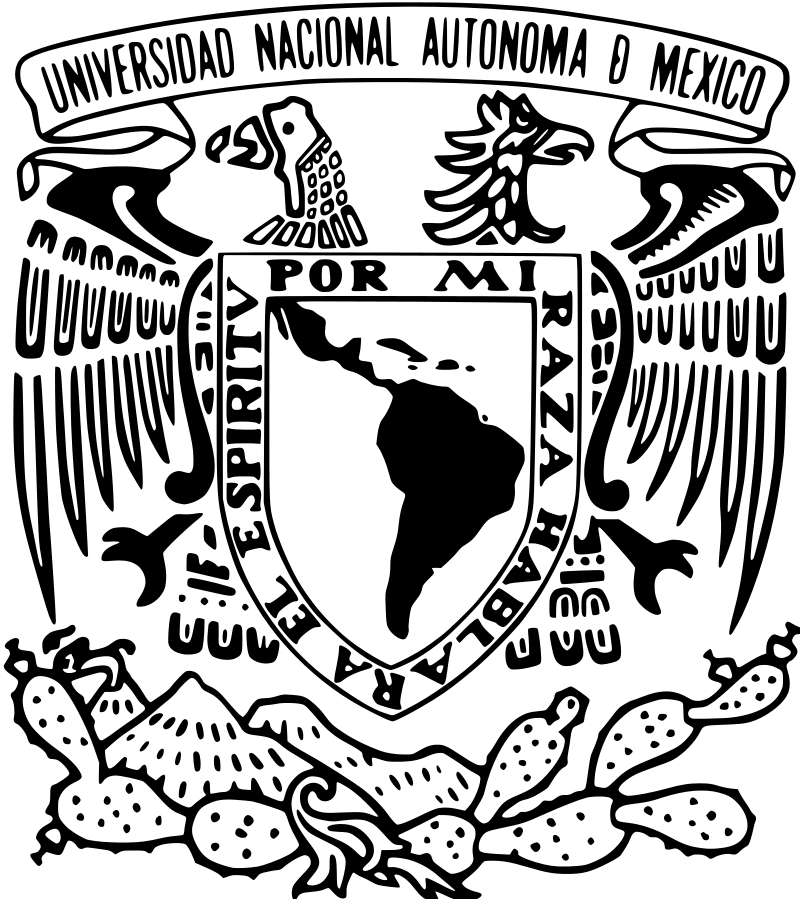
\includegraphics[width=4cm]{escudoUNAM_negro.png}
		% };

		\node[anchor=north east, inner sep=30] at (current page.north east) {
			
\includegraphics[width=3.5cm, height=4cm]{escudoFI_color.png}
		};
		% \node[anchor=north east, inner sep=30] at (current page.north east) {
		% 	
\includegraphics[width=4cm]{escudoFI_negro.png}
		% };
	\end{tikzpicture}

	\begin{center}
		\vspace*{2cm}

		\LARGE
		\textbf{Universidad Nacional Autónoma de México}\\
		Facultad de Ingeniería\\

		\vspace{1.5cm}

		\LARGE
		\textbf{Materia:} Organización Y Arquitectura de Computadoras\\
		\textbf{Profesor:} M.I. José Antonio de Jesús Arredondo Garza\\

		\vspace{1.5cm}

		\Huge
		\textbf{Práctica 1}\\
		\LARGE
		Raíz Cuadrada\\

		\vspace{1.5cm}

		\Large
		\begin{tabular}{|p{0.33\textwidth}|p{0.67\textwidth}|}
			\hline
			\textbf{No. de Cuenta} & \textbf{Nombre} \\
			\hline
			320068234 & Ayala Hernández María Fernanda \\
			\hline
			320335163 & Salazar Islas Luis Daniel \\
			\hline
			320078282 & Tepal Briseño Hansel Yael\\
			\hline
			320223822 & Ugartechea González Luis Antonio \\
			\hline
		\end{tabular}
		\vspace{1cm}

		\LARGE
		\textbf{Fecha de entrega:} <fecha\_entrega>\\
		\vspace{0.5cm}
		\Huge
		\textbf{Calificación:} \underline{\hspace{3cm}}
		\vspace{2.5cm}
	\end{center}
\end{titlepage}


\section{Objetivo}
En esta práctica se implementó una función para calcular la raíz entera de un número mediante la resta sucesiva de números impares. La idea principal es que la suma de los primeros $n$ números impares es $n^2$, por lo que al restar $1, 3, 5, 7, \dots$ se puede contar cuántas restas fueron necesarias para llegar a cero o a un valor menor.

\section{Desarrollo}

El desarrollo dela práctica consistió en implementar la función de raíz entera en dos lenguajes: MicroPython y ensamblador ARM. La función toma un número entero positivo y devuelve su raíz entera.

El algoritmo funciona de la siguiente manera:
\begin{itemize}
    \item Inicializa el resto con el valor original.
    \item Resta secuencialmente $1, 3, 5, 7, \dots$
    \item Cada resta exitosa representa una unidad de la raíz.
    \item Cuando el resto ya no alcanza al siguiente número impar, se termina y se
          devuelve el contador.
\end{itemize}

Por ejemplo, para $x=25$: $$25 - 1 - 3 - 5 - 7 - 9 = 0$$ Se realizaron 5
restas, por lo que $\lfloor \sqrt{25} \rfloor = 5$.

\section{Implementación en Python}

La implementación directa en MicroPython permite probar la lógica de manera sencilla. La función \texttt{py\_odd\_sqrt} recibe un número entero y devuelve su raíz entera.

\lstinputlisting[style=pythonstyle, firstline=37, lastline=47, caption={Implementación principal en Python}]{source/practica_01.py}

\section{Implementación en ARM}

La función ARM realiza el mismo procedimiento en lenguaje ensamblador, usando
registros para llevar el valor restante, el número impar actual y el contador
de la raíz. La lógica es equivalente a la versión en Python, pero optimizada
para ejecutarse directamente en la placa con la función \texttt{odd\_sqrt}.

\lstinputlisting[style=pythonstyle, firstline=17, lastline=33, caption={Implementación principal en ARM}]{source/practica_01.py}

\section{Pruebas y Validación}

Esta sección de código ejecuta una serie de pruebas en donde se compara la salida de el calculo obtenido para la solución en Python y la solución en ARM con una serie de valores esperados. Se imprimen los resultados de cada prueba, indicando si la prueba pasó o falló.

\lstinputlisting[style=pythonstyle, firstline=50, lastline=93, caption={Validación de casos de prueba en Python}]{source/practica_01.py}

\section{Ejecución en la Raspberry Pi Pico}

El archivo principal se puede cargar a la placa con el siguiente comando desde la carpeta raíz del proyecto:

\begin{lstlisting}[style=bashstyle]
./upload.sh practica_01/source/practica_01.py
\end{lstlisting}

El contenido del script que realiza esta ejecución es el siguiente:

\lstinputlisting[style=bashstyle, caption={Script de carga a la Pico}]{../upload.sh}

Este script:
\begin{itemize}
    \item valida que el archivo exista,
    \item libera el puerto si está ocupado,
    \item copia el programa a la Pico como \texttt{:main.py},
    \item y lo ejecuta inmediatamente con \texttt{mpremote}.
\end{itemize}

\section{Resultados}

La salida real obtenida al ejecutar el programa se muestra a continuación:

\lstinputlisting[style=bashstyle, caption={Salida generada por la práctica}]{source/output.txt}

\section{Conclusión}

La práctica demostró que la raíz entera puede obtenerse de manera eficiente a
partir de la suma de números impares. La versión en Python permite entender
claramente el procedimiento, mientras que la versión en ARM confirma la
viabilidad de la misma lógica en un entorno embebido.

%\section{Bibliografía}

\begin{biblio}
	% for: https://sistemasmultibasededatos.blogspot.com/
	\item Esquivel Martinez H. (2021, Noviembre 28). \textit{SISTEMAS MULTIBASE DE DATOS} [Online]. Disponible en: \newline \url{https://sistemasmultibasededatos.blogspot.com/}
\end{biblio}

\end{document}
